
\begin{frame}{Bases logiques}
    \begin{itemize}
        \item Logique du premier ordre sans symbole fonctionnel ;
        \item les objets sont des variables et les constantes ;
        \item les relations entre les objets sont faites par des prédicats ;
        \item un atome est de la forme $p(t_1,\ldots,t_n)$, avec $p$ un prédicat d'arité $n$ et des termes $t_i$ ;
        \item Une conjonction d'atomes sera représentée par un ensemble d'atomes ;
    \end{itemize}
    
    \begin{block}{Exemple}
        $\exists X, p(a,b) \land p(b,X)$ devient $\{p(a,b),p(b,X)\}$
    \end{block}
\end{frame}

\begin{frame}{Homomorphisme}
    \begin{block}{Homomorphisme d'un ensemble d'atomes dans un autre} Soit $S$ et $S'$, deux ensembles d'atomes. Un homomorphisme est une substitution $h$ des variables de $S$ par des termes de $S'$ telle que $h(S) \subseteq S'$.
    %Si on voit les ensembles d'atomes comme une conjonction d'atomes fermée existentiellement, alors $S$ s'envoie par homomorphisme dans $S'$ si et seulement si $S$ est conséquence logique de $S'$. Ceci explique pourquoi l'homomorphisme est la notion fondamentale pour le cadre que nous étudions. En particulier deux ensembles d'atomes sont équivalents si chacun s'envoie dans l'autre par homomorphisme. Ici, on le note $S \rightarrow S'$.
    \end{block}
    \begin{block}{Propriété}
        $\exists h, h(S) \subseteq S' \Leftrightarrow S' \vDash S$
    \end{block}
    \begin{block}{Exemple}
        $A = \{p(Z,b),p(b,Y)\}$\\
        $B = \{p(a,b),p(b,X)\}$ \\
        Il existe un homomorphimse $h$ tel que $h(A) \subseteq B$ : $h = \{(Z \mapsto a), (Y \mapsto X)\}$.
    \end{block}
\end{frame}

\begin{frame}[fragile]{Représentations d'un ensemble d'atomes}
Dans cette présentation, 2 représentations d'un ensemble d'atomes sont utilisées : graphe biparti et graphe orienté (arité < 2).

\begin{block}{Graphe biparti représentant $\mathcal{F} = \{p(a,b,X), q(b,X), p(X,Y,a)\}$}
\begin{asy}
// préambule asymptote
usepackage("amsmath,amssymb");
usepackage("inputenc","utf8");
usepackage("icomma");
// code figure
unitsize(1cm,1cm);
object sommet0=draw(Label("q"),ellipse,(0,0),NoFill);
object sommet1=draw(Label("X"),box,(2,0),NoFill);
object sommet2=draw(Label("Y"),box,(6,0),NoFill);
object sommet3=draw(Label("b"),box,(0,-2),NoFill);
object sommet4=draw(Label("a"),box,(4,-2),NoFill);
object sommet5=draw(Label("p"),ellipse,(2,-2),NoFill);
object sommet6=draw(Label("p"),ellipse,(4,0),NoFill);
add(new void(picture pic, transform t) {
path arete01=point(sommet0,dir(degrees((2,0),true)),t){dir(degrees((2,0),true))}..point(sommet1,dir(180+degrees((2,0),true)),t);
draw(pic,arete01);
label(pic,scale(.7)*"2",relpoint(arete01,.5),Relative(dir(90+degrees((2,0),true))),Fill(1,white));
path arete03=point(sommet0,dir(degrees((0,-2),true)),t){dir(degrees((0,-2),true))}..point(sommet3,dir(180+degrees((0,-2),true)),t);
draw(pic,arete03);
label(pic,scale(.7)*"1",relpoint(arete03,.5),Relative(dir(90+degrees((0,-2),true))),Fill(1,white));
path arete15=point(sommet1,dir(degrees((0,-2),true)),t){dir(degrees((0,-2),true))}..point(sommet5,dir(180+degrees((0,-2),true)),t);
draw(pic,arete15);
label(pic,scale(.7)*"3",relpoint(arete15,.5),Relative(dir(90+degrees((0,-2),true))),Fill(1,white));
path arete16=point(sommet1,dir(degrees((2,0),true)),t){dir(degrees((2,0),true))}..point(sommet6,dir(180+degrees((2,0),true)),t);
draw(pic,arete16);
label(pic,scale(.7)*"1",relpoint(arete16,.5),Relative(dir(90+degrees((2,0),true))),Fill(1,white));
path arete26=point(sommet2,dir(degrees((-2,0),true)),t){dir(degrees((-2,0),true))}..point(sommet6,dir(180+degrees((-2,0),true)),t);
draw(pic,arete26);
label(pic,scale(.7)*"2",relpoint(arete26,.5),Relative(dir(90+degrees((-2,0),true))),Fill(1,white));
path arete35=point(sommet3,dir(degrees((2,0),true)),t){dir(degrees((2,0),true))}..point(sommet5,dir(180+degrees((2,0),true)),t);
draw(pic,arete35);
label(pic,scale(.7)*"2",relpoint(arete35,.5),Relative(dir(90+degrees((2,0),true))),Fill(1,white));
path arete45=point(sommet4,dir(degrees((-2,0),true)),t){dir(degrees((-2,0),true))}..point(sommet5,dir(180+degrees((-2,0),true)),t);
draw(pic,arete45);
label(pic,scale(.7)*"1",relpoint(arete45,.5),Relative(dir(90+degrees((-2,0),true))),Fill(1,white));
path arete46=point(sommet4,dir(degrees((0,2),true)),t){dir(degrees((0,2),true))}..point(sommet6,dir(180+degrees((0,2),true)),t);
draw(pic,arete46);
label(pic,scale(.7)*"3",relpoint(arete46,.5),Relative(dir(90+degrees((0,2),true))),Fill(1,white));
});
shipout(bbox(0.1cm,0.1cm,white));
\end{asy}
\end{block}

\begin{block}{Graphe orienté représentant $\mathcal{F} = \{p(a,X), q(X,a), p(X,Y)\}$}
\begin{asy}
// préambule asymptote
usepackage("amsmath,amssymb");
usepackage("inputenc","utf8");
usepackage("icomma");
// code figure
unitsize(1cm,1cm);
object sommet0=draw(Label("a"),ellipse,(0,0),NoFill);
object sommet1=draw(Label("X"),ellipse,(2,0),NoFill);
object sommet2=draw(Label("Y"),ellipse,(4,0),NoFill);
add(new void(picture pic, transform t) {
path arete01=point(sommet0,dir(degrees((2,0),true)),t){dir(25+degrees((2,0),true))}..point(sommet1,dir(180+degrees((2,0),true)),t);
draw(pic,arete01,Arrow);
label(pic,scale(.7)*"p",relpoint(arete01,.5),Relative(dir(90+degrees((2,0),true))),Fill(1,white));
path arete10=point(sommet1,dir(degrees((-2,0),true)),t){dir(25+degrees((-2,0),true))}..point(sommet0,dir(180+degrees((-2,0),true)),t);
draw(pic,arete10,Arrow);
label(pic,scale(.7)*"q",relpoint(arete10,.5),Relative(dir(90+degrees((-2,0),true))),Fill(1,white));
path arete12=point(sommet1,dir(degrees((2,0),true)),t){dir(degrees((2,0),true))}..point(sommet2,dir(180+degrees((2,0),true)),t);
draw(pic,arete12,Arrow);
label(pic,scale(.7)*"p",relpoint(arete12,.5),Relative(dir(90+degrees((2,0),true))),Fill(1,white));
});
shipout(bbox(0.1cm,0.1cm,white));
\end{asy}
\end{block}


\end{frame}


\begin{frame}{Base de connaissances}
    \begin{block}{Base de connaissances}
        Elle est composée d'une base de faits, qui est un ensemble d'atomes, et d'un ensemble de règles        Elle est composée d'une base de faits $\mathcal{F}$, qui est un ensemble d'atomes, et d'un ensemble de règles $\mathcal{R}$.

.
    \end{block}
    
    \begin{block}{Exemple}
        $\mathcal{KB} = (\mathcal{F}, \mathcal{R})$
        \\ $\mathcal{F} = \{estHumain(socrate)\}$
        \\ $\mathcal{R} = \{r_1 = estHumain(X) \rightarrow estMortel(X)\}$.
    \end{block}
\end{frame}

\begin{frame}{Règles}
    \begin{block}{Règle}
        De la forme $\mbox{corps} \rightarrow \mbox{tête}$ où le corps et la tête sont des ensembles d'atomes.
    \end{block}
    
    \begin{block}{Règle Datalog}
        Les termes du corps et de la tête sont des constantes ou sont des variables quantifiées universellement.
        \par Exemple : $\forall X, p(a,X) \rightarrow p(X,a)$
    \end{block}
    
    \begin{block}{Règle existentielle}
        Pareil que Datalog, mais en plus, les variables présentes dans la tête mais pas dans le corps sont quantifiées existentiellement.
        \par Exemple : $\forall X, p(a,X) \rightarrow \exists Y, p(X,Y)$
    \end{block}
\end{frame}

\begin{frame}{Redondances}
    \begin{block}{Redondance}
    Un ensemble d'atomes S est redondant s'il existe un homomorphisme de S dans l'un de ses sous-ensembles stricts.
    \end{block}
    \begin{block}{Core}
    Un \textit{core} est un ensemble d'atomes non redondant.\\
    $Core(S)$ : sous-ensemble minimal de S équivalent à S.
    \end{block}
    \begin{block}{Exemple}
        $A = \{p(a,b),p(a,Y)\}$ contient une redondance. \\ 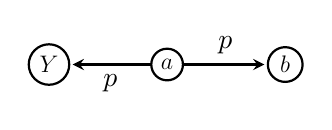
\begin{tikzpicture}[->,>=stealth,shorten >=1pt,auto,node distance=2.5cm,
                thick,main node/.style={circle,draw,font=\Large\bfseries,scale=0.6}]
            \node[main node] (3) {$Y$};
            \node[main node] (1) [right of=3] {$a$};
            \node[main node] (2) [right of=1] {$b$};
            \path
                (1) edge node {$p$} (2)
                (1) edge node {$p$} (3);
        \end{tikzpicture}\\ 
        $Core(A) = \{p(a,b)\}$ \\
        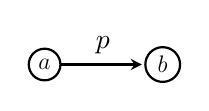
\begin{tikzpicture}[->,>=stealth,shorten >=1pt,auto,node distance=2.5cm,
                thick,main node/.style={circle,draw,font=\Large\bfseries,scale=0.6}]
            \node[main node] (1) {$a$};
            \node[main node] (2) [right of=1] {$b$};
            \path
                (1) edge node {$p$} (2);
        \end{tikzpicture}\\
        
    \end{block}
\end{frame}